As mentioned in \autoref{sec:crosslib:alignments:manually}, we had two students (Colin Rothgang and Yufei Liu) collect alignments between various theorem prover libraries. In the course of this project, they also developed interface theories for the symbols they aligned.

As a basis for this experiment, they used the foundational theory for the Math-in-the-Middle archive, a simplified excerpt of which is shown in \autoref{fig:mmtlogic}, as an interface for basic logical constants.

\begin{mmtcode}[caption= {An Interface Theory for Logic in \mmt\protect\footnotemark},label=fig:mmtlogic]
theory Logic : lfx:/TypedHierarchy?LFHierarchy =
	 // the type of booleans, i.e., all formulas are represented as terms of LF-type $prop$ ❙
	 prop 	: type ❘ @ bool  ❙
	 rule rules?BooleanLiterals ❙

	 ded 	: prop ⟶ type			❘ # ⊦ 1 prec -500 ❘ role Judgment ❙
	 
	 // Equality on terms. The type A is left implicit and can be inferred by MMT ❙
	 eq 	: {A:𝒰 100} A ⟶ A ⟶ bool	❘ # 2 ≐ 3 prec -5 ❘ role Eq ❙
	 
	 not  	: bool ⟶ bool 			❘ # ¬ 1 prec -100 ❙
	 neq 	: {A: 𝒰 100} A ⟶ A ⟶ prop	❘ # 2 ≠ 3 prec -5 ❙
	 and  	: bool ⟶ bool ⟶ bool		❘ # 1 ∧ 2 prec -110 ❙
	 or 	: bool ⟶ bool ⟶ bool		❘ # 1 ∨ 2 prec -120 ❙
	 impl	: bool ⟶ bool ⟶ bool		❘ # 1 ⇒ 2 prec -130 ❙
	 iff 	: bool ⟶ bool ⟶ bool		❘ # 1 ⇔ 2 prec -140 ❙
   
	 forall : {A : 𝒰 100} (A ⟶ bool) ⟶ bool	❘ # ∀ 2 prec -100❙
	 exists : {A : 𝒰 100} (A ⟶ bool) ⟶ bool	❘ # ∃ 2 prec -100 ❙
\end{mmtcode}
\footnotetext{\url{https://gl.mathhub.info/MitM/Foundation/blob/master/source/math.mmt}}

This theory actually includes most of the features presented in \autoref{ch:lf}, in order to be as flexible as possible in formalizing content -- although most of them were not yet available when the experiment described in this section was originally done.

%\begin{figure}[ht]\centering
%  \fbox{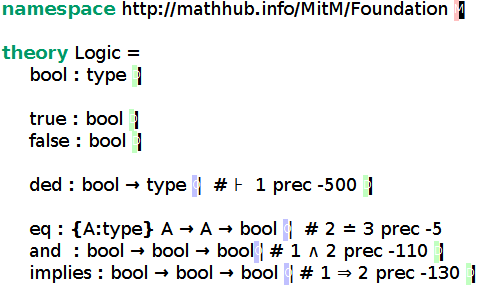
\includegraphics[width=0.45\textwidth]{img/trans-logic}}
%  \caption{An interface theory for logic in \mmt}\label{fig:mmtlogic}
%\end{figure}

%Here, a new theory \expr{Logic} is declared with URI \textsf{http://mathhub.info/MitM/Foundation?Logic}, which is composed of the namespace declared in the first line and the name of the theory. Afterwards, three constants are declared and given a type; namely the type of booleans \expr{bool} of type \expr{type}. The symbol \expr{type} is provided via a logical framework. The constants \expr{true} and \expr{false} are declared to be of type \expr{bool}.
%
%In general, \mmt constants have the form \expr{c [:TYPE] [=DEF] [\#NOT]}, though we will not need definitions in this paper. The individual components (type, definition, notation, respectively) are all optional and can be provided in any order.
%
%The symbol \expr{ded} will serve as a function from propositions to the type of their proofs to make use of the Curry-Howard correspondence. It is given the appropriate type \expr{bool \to type} and a notation \expr{\vdash\textsf{ 1 }}. The latter allows for writing \expr{\vdash\textsf A} for the type of proofs of a proposition $A$. Furthermore, the notation is provided with a precedence, to allow for omitting brackets.
%
%The next symbols provide a typed equality and the basic logical connectives. The curly braces denote the dependent function type, providing for example \expr{eq} with the type $\expr{\prod_{\textsf{A:type}}\textsf A\to\textsf A\to\textsf{bool}}$. The notation \expr{2 \doteq 3} omits the first argument \expr{A:type}, leaving it implicit and to be inferred by the system.
%
%\paragraph{}
%We can use this theory as one (out of many possible) meta-theory for various interface theories.

\subsection{Example: Natural Numbers}

\autoref{fig:natinterface} shows an example of a simple theory of natural numbers, using the theory \expr{Logic} and the symbols declared therein. Note, that this theory is basically an implementation of the Peano axioms, which can be seen as the interface theory for all possible definitions of a concrete set (or type) of ``the'' natural numbers.

\begin{mmtcode}[caption= {An (excerpt of an) interface theory for natural numbers with \texttt{Logic} as meta-theory\protect\footnotemark},label=fig:natinterface]
theory Naturals : fnd:?Logic =
	zero		:  ℕ ❘ = 0 ❙
  	successor	:  ℕ ⟶ ℕ 		❘ # S 1 ❙
	plus		:  ℕ ⟶ ℕ ⟶ ℕ 		❘ # 1 + 2 ❙
	times		:  ℕ ⟶ ℕ ⟶ ℕ 		❘ # 1 ⋅ 2 ❙
	leq		:  ℕ ⟶ ℕ ⟶ bool 	❘ # 1 ≤ 2 ❙
	
	Induction	: {P} ⊦ P zero ⟶ ({n} ⊦ P n ⟶ ⊦ P (S n)) ⟶ ⊦ ∀ P ❙
	Succ_inj	: {n:ℕ,m:ℕ} ⊦ (S n) ≐ (S m) ⊦ n ≐ m ❙
	
	plus_zero	: {n} ⊦ (n + zero) ≐ n ❘ role Simplify ❙
	plus_succ	: {n,m} ⊦ (n + (S m)) ≐ S (n + m) ❘ role Simplify ❙
	
	times_zero	: {n} ⊦ (n ⋅ zero) ≐ zero ❘ role Simplify ❙
	times_succ	: {n,m} ⊦ (n ⋅ (S m)) ≐ ((n ⋅ m) + n) ❙
\end{mmtcode}
\footnotetext{\url{https://gl.mathhub.info/MitM/interfaces/blob/master/source/Math/Numbers.mmt}}
%\begin{figure}[ht]\centering
%  \fbox{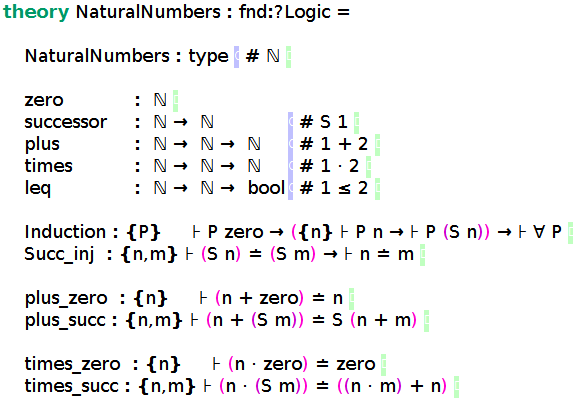
\includegraphics[width=0.5\textwidth]{img/trans-natinterface}}
%  \caption{An (excerpt of an) interface theory for natural numbers with \textsf{Logic} as meta-theory}\label{fig:natinterface}
%\end{figure}

In Mizar~\cite{mizar}, which is based on Tarski-Grothendieck set theory, the set of natural numbers \expr{NAT} is defined as \textsf{omega}, the set of finite ordinals. Arithmetic operations are defined directly on those.

In contrast, in PVS (see \autoref{ch:import:pvs}) natural numbers are defined as a specific subtype of the integers, which in turn are a subtype of the rationals etc. up to an abstract type \expr{number} which serves as a maximal supertype to all number types. The arithmetic operations are inherited from a subtype \expr{number\_field} of \expr{number}.

These are two fundamentally different approaches to describe and implement an abstract mathematical concept, but for all practical purposes the concept they describe is the same; namely the natural numbers. The interface theory for both variants would thus only contain the symbols that are relevant to the abstract concept itself, independent of their specific implementation -- hence, things like the type of naturals, the arithmetic operations and the Peano axioms. The interface theory thus provides everything we need to work with natural numbers, and at the same time everything we know about them independently of the logical foundation or their specific implementation within any given formal system.

\paragraph{}However, there is an additional layer of abstraction here, namely that in stating that the natural numbers in Mizar are the finite ordinals we have already ignored the system dialect (in the sense of \autoref{lbl:dialect} in the introduction to this chapter). This step of abstraction (from the concrete definition using only Mizar-specific symbols) yields another interface theory for finite ordinals, which in turn can be aligned not just with Mizar natural numbers, but also e.g. with MetaMath~\cite{MetaMath:on}, which is built on ZFC set theory.

\autoref{fig:intgraph} illustrates this situation. Blue arrows point from more detailed theories to their interfaces. The arrows from PVS or Mizar to interfaces merely strip away the system dialects; the arrows within Interfaces abstract away more fundamental differences in definition or implementation.

\begin{figure}%[hbp]
\begin{center}
\resizebox{0.6\textwidth}{!}{
\begin{tikzpicture}

\node (PVS) at (1,8.5) {PVS};

\node (PVNat) at (1,7) {\textsf{Nat}};
\node (PVdots) at (1,5) {$\vdots$};
\node (PVnf) at (1,3) {\textsf{number\_field}};
\draw[\arrowtipmono-\arrowtip] (PVnf) -- (PVdots);
\draw[\arrowtipmono-\arrowtip] (PVdots) -- (PVNat);
 \node[draw,thick,fit=(PVNat) (PVdots) (PVnf),
                   rounded corners=.55cm, inner sep=5pt] (PVScloud) {};

\node (Int) at (6,8.5) {Interfaces};

\node (ST) at (7.6,4.2) {Ordinals};

\node (Reals) at (4.7,4.8) {\textsf{Numbers}};
\node (Nat) at (4.7,6) {$\mathbb N$};
\draw[\arrowtipmono-\arrowtip] (Reals) -- (Nat);

\node (FOrd) at (7.2,5.5) {Finite Ordinals};

\node (PA) at (6,7) {Peano Axioms};
\draw[->,blue] (FOrd) -- (PA);
\draw[->,blue] (Nat) -- (PA);
\draw[\arrowtipmono-\arrowtip] (ST) -- (FOrd);

 \node[draw,thick,fit=(ST) (Reals) (Nat) (FOrd) (PA),
                   rounded corners=.55cm, inner sep=10pt] (PVScloud) {};

\node (Miz) at (11,8.5) {Mizar};

\node (MNat) at (11,7) {\textsf{Nat}};
\node (MOrd) at (11,3) {\textsf{Ordinals}};
\draw[\arrowtipmono-\arrowtip] (MOrd) -- (MNat);

 \node[draw,thick,fit=(MNat) (MOrd),
                   rounded corners=.55cm, inner sep=5pt] (PVScloud) {};

\draw[->,blue] (MOrd) -- (ST);
\draw[->,blue] (PVNat) -- (Nat);
\draw[->,blue] (PVnf) -- (Reals);
\draw[->,blue] (MNat) -- (FOrd);


\end{tikzpicture}
}
\end{center}
\caption{A Graph Showing Different Theories for Natural Numbers}\label{fig:intgraph}
\end{figure}

\paragraph{} Consider again \autoref{fig:natinterface}, a possible interface theory for natural numbers. Note, that symbols such as \expr{leq} \emph{could} be defined, but don't actually need to be. Since they are only interfaces, all we need is for the symbols to exist. 
 
 In fact, the more abstract the interface, the less we \emph{want} to define the symbols -- given that there's usually more than one way to define symbols, definitions are just one more thing we might want to abstract away from completely. There are exceptions to this -- note that the symbol \expr{zero} is actually defined as the literal $0$.\footnote{See \autoref{sec:lf:lfx:literals} for more on Literals in \mmt.} This is because literals themselves are mere \mmt terms, but not symbols with a stable \mmt-URI, which we need for alignments. On the other hand, not having literals excludes those systems where literals are actually used. In this case, providing a definition to the symbols enables aligning both systems with and without literals.\medskip
 
 The symbols in this interface theory can then be aligned either with symbols in other formal systems directly, or with additional interfaces in between, such as a theory for Peano arithmetic, or the intersection of all inductive subsets of the real numbers, or finite ordinals or any other possible formalization of the natural numbers.

\subsection{Additional Interface Theories}\label{subsec:crosslib:interfaces}

The foundation independent nature of \mmt allows us to implement interface theories with almost arbitrary levels of detail and for vastly different foundational settings.

We have started a repository of interface theories specifically for translation purposes~\cite{MitMInter:on} and also aligned to already existing interfaces (as in the case of arithmetics, see below) in a second and third \mathhub repository~\cite{mitm:smglom:on} and~\cite{mitm:foundation:on} extending them when necessary. \medskip

Crucially, this interface repository contains interface theories for basic type-related symbols like the function type constructors (see \autoref{fig:typeinterface}\footnote{This interface theory, like most formalizations of foundations, uses types as terms (via the symbols \expr{tp} and \expr{tm}), whereas the interface theories above (like \expr{NaturalNumbers}) use the universe of types provided by the logical framework directly. During translation, special \emph{higher-order abstract syntax rules} take care of eliminating or inserting the corresponding symbols appropriately to make aligning between the two formalization levels possible (see \autoref{sec:lf:prelim:hoas}).}), that are aligned with the respective symbols in HOL Light and PVS. These symbols are so basic as to be primitive in systems based on type theory, and consequently they occur in the vast majority of expressions. To have these symbols aligned is strictly necessary to get any further use of alignments off the ground.

\begin{mmtcode}[caption= {Interface Theories for Type-Theoretical Foundations\protect\footnotemark},label=fig:typeinterface]
theory TypeSystem : ur:?LF =
	tp : type ❙
	tm : tp ⟶ type ❙
❚

theory SimpleFunctionTypes : ?TypeSystem =
	Arrowtp : tp ⟶ tp ⟶ tp ❘ # 1 ⟹ 2 ❙
	Applytp : {A,B} tm (A ⟹ B) ⟶ tm A ⟶ tm B ❘ # 3 @ 4 ❘ ## 3 4 ❙
	Lambdatp : {A,B} (tm A ⟶ tm B) ⟶ tm (A ⟹ B) ❘ # λ 3 ❙
❚
	
theory DependentFunctionTypes : ?TypeSystem =
	Pitp : {A} (tm A ⟶ tp) ⟶ tp ❘ # Π 2 ❙
	Applytp : {A,B} tm (Pitp A B) ⟶ {x: tm A} tm (B x) ❘ # 3 @ 4 ❘ ## 3 4 ❙
	Lambdatp : {A,B} ({x: tm A} tm (B x)) ⟶ tm (Π B) ❘ # λ 3 ❙
	structure simple : ?SimpleFunctionTypes =
		Arrowtp = [A,B] Pitp A ([x]B) ❙
		Applytp = [A,B][f][a] Applytp A ([x]B) f a ❙
		Lambdatp = [A,B][f] Lambdatp A ([x]B) f ❙
	❚
❚


\end{mmtcode}
\footnotetext{\url{https://gl.mathhub.info/MitM/interfaces/blob/master/source/TypeSystem.mmt} and \url{https://gl.mathhub.info/MitM/interfaces/blob/master/source/TypeConstructors.mmt}}

%\begin{figure}[ht]\centering
%  \fbox{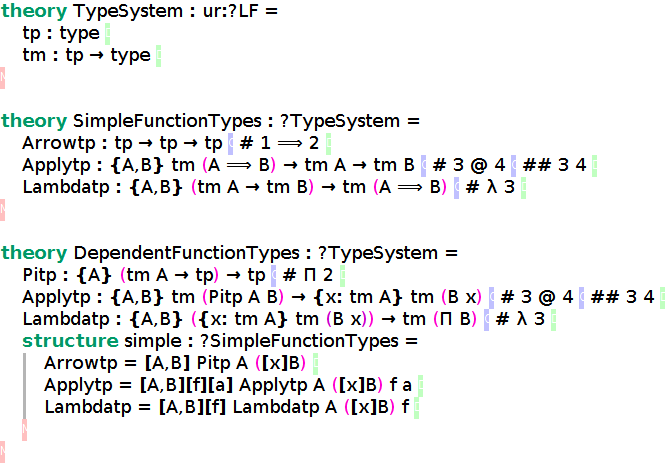
\includegraphics[width=0.6\textwidth]{img/trans-typeinterface}}
%  \caption{Interface theories for type-theoretical foundations\label{fig:typeinterface}}
%\end{figure}

Here, a \emph{structure} is used to include the theory for simple function types in the theory for dependent function types, while providing definitions for the symbols in terms of the latter. This automatically yields a translation from the simple to the dependent variant and demonstrates the advantage of using interface theories for translations: The general problem of converting between (systems using) simple and dependent function types is lifted to the level of the interface theories, where we can use theory morphisms (such as structures) to specify the appropriate translation once and for all; independent of any specific external system.\medskip

\autoref{tbl:alignmenttotal} shows the total number of alignments the students found for PVS, HOL Light and Mizar. The following are some additional examples of mathematical areas covered by the resulting interface theories. The numbers here reflect the result of the student experiment and refer to the number of symbols actually used for alignments therein; the theories themselves have been partially adapted and significantly extended by now:

  \paragraph{Calculus} contains the following 3 subinterfaces:
  %\begin{itemize}
  	\subparagraph{Limits} contains 17 symbols related to sequences and limits, including \expr{metric\_space} and \expr{complete} (metric spaces and their completeness). %We currently have 8 alignments to HOL Light and 9 to Mizar.Neither true, nor belongs here. We have alignments to all three systems. Amonh them there are 7 alignments to Hol Light and 15 to Mizar (even though one alignment is duplicated, as there are two corresponding synonimical HOL Light symbols)
  	\subparagraph{Differentiation} contains 4 symbols, namely differentiability in a point and on a set and the derivative in a point and as a function
  	\subparagraph{Integration} contains 6 symbols, namely integrability and the integral over a set for Riemann, Lebesgue and Gauge-integration.
  \paragraph{} For \textbf{Arithmetics} we use the already existing theories from ~\cite{mitm:smglom:on}. It contains interfaces for below number arithmetics (each split into two interfaces for the basic number type definitions and the arithmetics on them). 
  %\begin{itemize}
    \subparagraph{Complex Numbers} contains 11 symbols for complex numbers aligned to their counterparts in HOL Light, PVS and Mizar. Besides the usual arithmetic operations similar to \expr{NaturalNumbers}, it contains \expr{i} (the imaginary unit), \expr{abs} (the modulus of a complex number) and \expr{Re}, \expr{Im}  (the real and imaginary parts of a complex number). %11 of the symbols are aligned with HOL Light, 7 with Mizar and 10 with PVS.
    \subparagraph{Integers} contains 9 symbols for the usual arithmetic operations on integers and for comparison between two integers. %Since HOL Light and PVS do not treat these as distinct symbols, we only aligned them with Mizar so far.
    \subparagraph{Natural Numbers} contains 21 symbols and is already described above. 
    \subparagraph{Real Numbers} contains 15 symbols, again very similar in nature to the other number spaces. % 13 of these are aligned with HOL Light and PVS and 10 with Mizar.
  %\end{itemize}
  \paragraph{Lists} contains the 13 most important symbols for lists, including \expr{head}, \expr{tail}, \expr{concat}, \expr{length} and \expr{filter} (filter a list using another list) as well as some auxiliary definitions. % We have 15 alignments to HOL Light (three of them are in a different theory in MitM) and 9 to PVS.
  There are no lists in Mizar, instead finite sequences are used. These however deserve their own interface.
  \paragraph{} For \textbf{Logic} we use the already existing theories in the~\cite{mitm:foundation:on} repository. It contains 9 symbols for boolean algebra that are all perfectly aligned to HOL Light, PVS and Mizar, and sometimes also to Coq.
  \paragraph{Sets} are also already existent in ~\cite{mitm:smglom:on}, split into many subtheories. 28 of the contained symbols have been aligned. sets contains symbols for typed sets as in a type theoretical setting, including axioms and theorems. Here we have the most alignments so far. It also contains the following two interfaces:
  %\begin{itemize}
  	\subparagraph{Relations} contains 23 symbols for alignments to relations and their properties, including orders. 
  	\subparagraph{Functions} contains 7 symbols for alignments to functions and their relations, that are not already contained in relations. 
  %\end{itemize}
  \paragraph{Topology} contains 25 symbols for both general topological spaces as well as the standard topology on $\mathbb R^n$ specifically. %Since this yields additional difficulties, it will be examined in more detail in the next     section.
% \end{itemize}
 %\paragraph{} As additional examples, the interface theories for limits and sets can be found in Figures \ref{fig:anatheory} and \ref{fig:setstheory}.
 
 \paragraph{}
% the below sentence is not related to the topic here
%In order to translate expressions between libraries, one alignment in each library to an interface symbol is needed.
In order to translate an expression from one library to another, the concepts in the expression must at least exist in both libraries. This creates the need to inspect the intersection of the concepts in these libraries.
\autoref{tbl:intersectionConcepts} gives an overview of the library intersection for various interface theories.
\begin{table}[ht]\centering\footnotesize	
	\begin{tabular}{|c|c|c|c|c|}
		\hline Topic & 1 System & 2 Systems & 3 Systems & 4 Systems\\
		\hline \textsf{Algebra}& \textsf{17} & \textsf{9} & \textsf{5} & \textsf{0}\\
		\hline \textsf{Calculus}& \textsf{35} & \textsf{7} & \textsf{8} & \textsf{0}  \\
		\hline \textsf{Categories} & \textsf{4} & \textsf{5} & \textsf{0} & \textsf{0}\\
		\hline \textsf{Combinatorics}& \textsf{25} & \textsf{6} & \textsf{0} & \textsf{1}  \\
		\hline \textsf{Complex Numbers} & \textsf{10} & \textsf{5} & \textsf{3} & \textsf{3}\\
		\hline \textsf{Graphs} & \textsf{72} & \textsf{6} & \textsf{3} & \textsf{0}\\
		\hline \textsf{Integers}& \textsf{52 }& \textsf{2 }& \textsf{7} & \textsf{0} \\
		\hline \textsf{Lists}& \textsf{28} & \textsf{8} & \textsf{9} & \textsf{0} \\
		\hline \textsf{Logic}& \textsf{18} & \textsf{0} & \textsf{2}& \textsf{5} \\
		\hline \textsf{Natural Numbers} & \textsf{53} & \textsf{2} & \textsf{10}& \textsf{2}  \\
		\hline \textsf{Polynomials} & \textsf{12} & \textsf{0} & \textsf{0}& \textsf{0}  \\
		\hline \textsf{Rational Numbers} & \textsf{11} & \textsf{4} & \textsf{2}& \textsf{7}  \\
		\hline \textsf{Real Numbers}  & \textsf{9} & \textsf{3} & \textsf{5} & \textsf{5}\\
		\hline \textsf{Relations}  & \textsf{21} & \textsf{15} & \textsf{4} & \textsf{0}\\
		\hline \textsf{Sets}  & \textsf{56} & \textsf{10} & \textsf{9} & \textsf{10}\\
		\hline \textsf{Topology} & \textsf{62} & \textsf{2} & \textsf{8}& \textsf{0} \\
		\hline \textsf{Vectors} & \textsf{25} & \textsf{5} & \textsf{0}& \textsf{0} \\
		\hline \textbf{Sum}  & \textbf{510} & \textbf{91} & \textbf{79}& \textbf{33} \\ 
		\hline 
	\end{tabular}
	\caption{Number of Concepts Found in Exactly One, Two, Three or Four Systems}
	\label{tbl:intersectionConcepts}
\end{table}

\autoref{fig:mitmgraph} shows a small part of the theory graph of the \textsf{MitM} libraries. The full \textsf{MitM} theory graph can be explored on \mathhub\footnote{\url{https://mathhub.info/mh/mmt/graphs/tgview.html?graphdata=MitM}}.

\begin{figure}[ht]\centering
  \fbox{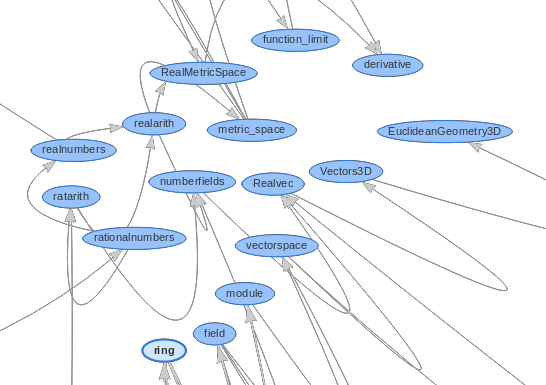
\includegraphics[width=0.6\textwidth]{img/trans-mitmgraph}}
  \caption{A Small Part of the MitM Theory Graph}\label{fig:mitmgraph}
\end{figure}

%\begin{itemize}
%	\item Lists, containing symbols for head, tail, concatenation, length, filter etc.
%	\item Calculus, containing symbols for sequences of real numbers, convergence, limit, monotonicity etc.
%	\item Typed sets, containing symbols for elementhood, intersection, union, the empty set and axioms/theorems like extensionality, transitivity of the subset relation etc.
%	\item Integers, containing similar symbols as the interface theory for natural numbers.
%\end{itemize}